\chapter{集合论}
虽然直到19世纪末德国数学家康托(Cantor)才创立了集合论,但是其实人们很早就开始使用集合的概念与运算了.
在《周易·系辞下》中有这么一句话:“上古结绳而治,后世圣人易之以书契.”
于是我们想到,古人在农业生产中始终有着对农产品(例如红枣、覆盆子、野兔、鲤鱼等)分类、计数的需要,即将同类的产品集中地放置,再用一个符号(绳结或算筹)表示这类产品的数量.

对于分类的标准的探索,或者说对于物的“同一性”与“差异性”的研究,也同样源远流长.
古希腊哲学家赫拉克利特(Heraclitus)也提出“太阳每天都是新的”“人不能两次踏进同一条河流”,并认为事物总是在变化的,观念上的同一的物也是不同的;后来,罗马哲学家普鲁塔克(Plutarchus)也提出了著名的忒修斯之船(The Ship of Theseus)悖论.
但是,即使椭圆、双曲线和抛物线在几何形态上存在天差地别,古希腊数学家阿波罗尼(Apollonius)仍将它们归作一类,看作相似的概念,并创立了《圆锥曲线论》.
为了解决上述问题,一组相对的哲学概念被提出来了,这就是“逻辑同一性”和“实在同一性”.
简单地说,实在同一性和逻辑同一性都是对事物关系的一种描述,实在同一性要求被比较的事物无法被区分,而逻辑同一性是指两个物在部分的属性上具备某种相同、相等或相似的关系.
以实在同一性和逻辑同一性作为分类的标准,我们就可以区分事物以构建对立关系,又可以混同事物以构建等价关系.

\section{朴素集合论}
\subsection{集合的概念}
\begin{definition}
\textbf{集合}(简称\textbf{集},Set)是指具有某种特定性质的事物的总体.
组成这个集合的事物称为该集合的\textbf{元素}(简称\textbf{元},Member或Element).
集合常用大写字母(如\(A,B,C,X,Y\)等)表示,元素常用小写字母(如\(a,b,c\)等)表示.

如果元素\(a\)是集合\(A\)的元素,就说“\(a\)\textbf{属于}\(A\)(\(a\) is a member of \(A\)或\(a\) belongs to \(A\))”,记作\(a \in A\);
如果\(b\)不是集合\(A\)的元素,就说“\(b\)\textbf{不属于}\(A\)(\(b\) is not a member of \(A\))”,记作\(b \notin A\).
\end{definition}

\begin{property}
集合具有三种特性:\begin{enumerate}
\item \textbf{确定性},即对于任意一个元素,要么它属于某个指定集合,要么它不属于该集合,二者必居其一;
\item \textbf{互异性},即同一个集合中的元素是互不相同的;
\item \textbf{无序性},即任意改变集合中元素的排列次序,它们仍然表示同一个集合.
\end{enumerate}
\end{property}

\begin{definition}
由不是集合的元素组成的集合,叫做\textbf{第一层集}.
把第一层集当作元素组成的集合,叫做\textbf{第二层集}(又称\textbf{系}).
\end{definition}

把集合的全体元素一一列举出来,用以表示集合的方法,称为\textbf{列举法}.
例如由\(n\)个元素\(\v{a}{n}\)组成的集合,可表示为\[
\Set{ \v{a}{n} }.
\]

\subsection{集合的关系与运算}
\begin{axiom}[外延公理]
如果集合\(A\)与集合\(B\)具有相同的元素,则称集合\(A\)与集合\(B\)\textbf{相等},记作\(A=B\),即\[
\forall A, \forall B \Bigl[
	\forall x \bigl( x \in A \iff x \in B \bigr)
	\implies A = B
\Bigr].
\]
\end{axiom}
外延性公理在英语中称作Extensionality Axiom,在德语中称作Axiom der Bestimmtheit.

\begin{axiom}[空集公理]
总存在这样一个集合,没有任何元素属于它,即\[
\exists A,\forall x( x \notin A ).
\]
\end{axiom}
空集公理在英语中称作Empty Set Axiom.

\begin{definition}
不含任何元素的集合称为\textbf{空集}(Empty set),记作\(\emptyset\).
\end{definition}
定义空集\(\emptyset\)时一定要注意两点:一是“空集”是否存在,这已由空集公理确保;二是“空集”是否唯一,这则由外延公理确保.
没有这两条公理的帮助,我们就不能说\(\emptyset\)是\cemph{定义良好的}.

\begin{example}
以空集为元素构成的集合\(\Set{\emptyset}\)不是空集,即\(\Set{\emptyset} \neq \emptyset\).
这是因为\(\emptyset \in \Set{\emptyset}\)但\(\emptyset \notin \emptyset\).
\end{example}

\begin{axiom}[对集公理]
对于任意集合\(u\)和\(v\),总存在一个集合\(B\),它的元素只有\(u\)和\(v\),即\[
\forall u, \forall v, \exists B, \forall x \bigl(
	x \in B \iff x = u \lor x = v
\bigr).
\]
\end{axiom}
对集公理在英语中称作Pairing Axiom.

在德语中把对集公理和空集公理并称为Axiom der Elementarmengen.

\begin{definition}
设\(A\)、\(B\)是两个集合,称集合\[
\Set{ A, B }
\]为\(A\)和\(B\)的\textbf{对集}(Pair set).
\end{definition}

\begin{axiom}[子集公理]
对于不涉及\(B\)的每一条命题公式\(\lambda\),下式是一条公理:\[
\forall A, \exists B, \forall x \bigl(
	x \in B \iff x \in A \land \lambda
\bigr).
\]
\end{axiom}
子集公理有时候也称作\textbf{分离公理},它在英语中称作Subset Axioms,在德语中称作Axiom der Aussonderung.
正如其名,该定理的作用就是从集合\(A\)中取出适合命题公式\(\lambda\)的元素,组合成新的集合\(B\).

由子集公理可知,除了用列举法表示集合以外,还可以通过说明集合中的元素具有的性质来确定集合,这种方法称为\textbf{描述法}.例如若集合\(M\)是由具有某种性质\(P\)的元素\(x\)的全体所组成的,就可表示为\[
M = \Set{ x \given x\ \text{具有性质}\ P }.
\]

利用描述法,我们可以重新定义空集如下:\[
\emptyset \equiv \Set{ x \given x \neq x },
\]\[
\Set{ u, v } \equiv \Set{ x \given x = u \lor x = v };
\]

\begin{theorem}
以所有集合为元素组成的集合不存在.
\begin{proof}
设\(A\)是一个集合,那么我们总可构造出一个不属于\(A\)的集合.记\[
B = \Set{ x \in A \given x \notin x },
\]那么有\[
B \in B \iff B \in A \land B \notin B.
\]

假设\(B \in A\),那么上式化为\[
B \in B \iff B \notin B,
\]矛盾,故\(B \notin A\).
\end{proof}
有的人可能会对是否存在以其本身为元素的集合抱有疑问,我们将在后面证明这是不可能的.
而根据这个结论,在上面的证明中,集合\(B\)实际上与集合\(A\)完全相同.
\end{theorem}

利用子集定理,我们可以进一步定义子集、真子集、交集等概念.
\begin{definition}
设\(A\)、\(B\)是两个集合,如果集合\(A\)的元素都是集合\(B\)的元素,则称\(A\)是\(B\)的\textbf{子集}(\(A\) is a Subset of \(B\)),记作\(A \subseteq B\)(读作\(A\)包含于\(B\),\(A\) is included in \(B\))或\(B \supseteq A\)(读作\(B\)包含\(A\),\(B\) includes \(A\)),即\[
\forall x \in A \bigl( x \in B \bigr) \iff A \subseteq B.
\]

若集合\(A \subseteq B\)且\(A \neq B\),则称\(A\)是\(B\)的\textbf{真子集}(Proper subset),记作\(A \subsetneqq B\).
\end{definition}

\begin{property}
任意集合都是其本身的子集,即\[
\forall A \bigl( A \subseteq A \bigr).
\]
\end{property}

\begin{property}
空集\(\emptyset\)是任何集合的子集,即\[
\forall A \bigl( \emptyset \subseteq A \bigr);
\]还是任何非空集合的真子集,即\[
\forall A \bigl( A \neq \emptyset \iff \emptyset \subsetneqq A \bigr).
\]
\end{property}

在学习了从属关系(\(\in\))和包含关系(\(\subseteq\))以后,切莫将两者搞混.
在讨论\(A \in B\)是否成立时,我们是将\(A\)作为一个整体,看它是不是\(B\)中的一个元素.
在讨论\(A \subseteq B\)是否成立时,我们要将\(A\)打开,检查它里面的所有元素是不是都是\(B\)中的元素.

\begin{theorem}
如果集合\(A\)与集合\(B\)互为子集,那么集合\(A\)与集合\(B\)相等,即\[
A \subseteq B \land B \subseteq A \iff A = B.
\]
\end{theorem}

\begin{axiom}[幂集公理]
对于任意集合\(A\),总存在这样一个集合——它的全部元素恰好是集合\(A\)的全部子集,即\[
\forall A, \exists B, \forall x ( x \in B \iff x \subseteq A ).
\]

像这样由集合\(A\)的所有子集(包括空集和集合\(A\)本身)构成的集合\(B\),称作集合\(A\)的\textbf{幂集}(Power set),记作\(\Powerset A\)(有的地方也记作\(2^A\)或\(\mathcal{P}A\)),即\[
\Powerset A \equiv \Set{x \given x \subseteq A}.
\]
\end{axiom}
幂集公理在英语中称作Power Set Axiom,在德语中称作Axiom der Potenzmenge.

空集公理、对集公理、并集公理、幂集公理并称\textbf{集合存在公理}(Set existence axioms).

\begin{example}
\(\Powerset \emptyset = \{ \emptyset \},%
\Powerset \Set{ \emptyset } = \{ \emptyset, \{ \emptyset \} \}\).
\end{example}

\begin{example}
对于任意集合\(A,B\),试分析\(\Powerset(A-B)\)与\(\Powerset A - \Powerset B\)是否相等.
\begin{solution}
集合\(\Powerset(A-B)\)包含集合\(A-B\)的所有子集,那么总有\(\emptyset\in\Powerset(A-B)\).
但是\(\emptyset\notin\Powerset A - \Powerset B\),所以\(\Powerset(A-B) \neq \Powerset A - \Powerset B\).
\end{solution}
\end{example}

\begin{axiom}[并集公理]
对于任意集合\(a\)和\(b\),总存在这样一个集合——它的元素要么属于\(a\),要么属于\(b\),即\[
\forall a, \forall b, \exists B, \forall x( x \in B \iff x \in a \lor x \in b ).
\]
\end{axiom}
上述公理在英语中称作Union Axiom, Preliminary Form.
并集公理在德语中称作Axiom der Vereinigung.

\begin{definition}[集合的交、并、差]
设集合\(A\)、\(B\).
称集合\[
\Set{ x \given x \in A \land x \in B }
\]为\(A\)和\(B\)的\textbf{交集}(简称\textbf{交},the intersection of \(A\) and \(B\)),记作\(A \cap B\).

称集合\[
\Set{ x \given x \in A \lor x \in B }
\]为\(A\)和\(B\)的\textbf{并集}(简称\textbf{并},the union of \(A\) and \(B\)),记作\(A \cup B\)或\(A+B\).

称\[
\Set{ x \given x \in A \land x \notin B }
\]为\(A\)和\(B\)的\textbf{差集}(the relative complement of \(B\) in \(A\)),记作\(A - B\)或\(A \setminus B\).
\end{definition}

\begin{definition}[全集、补集]
有时,我们研究某个问题限定在一个大的集合\(U\)中进行,所研究的其他集合都是\(U\)的子集.此时我们称集合\(U\)为\textbf{全集}(或\textbf{基本集}).设\(A \subseteq U\),则称\(U-A\)为\(A\)的\textbf{补集}(或\textbf{余集}),记作\(\overline{A}\)(或\(\complement_U A\),或\(A^C\)).
\end{definition}

我们可以进一步改善并集公理如下:
\begin{axiom}[并集公理']
对于任意集合\(A\),总存在一个集合\(B\),使得集合\(B\)中的所有元素都属于集合\(A\)中的元素,即\[
\forall x \bigl[
	x \in B \iff (\exists b \in A) x \in b
\bigr].
\]
\end{axiom}
在给出上述并集公理后,原本的并集公理就可以抛弃不用了.

\begin{theorem}
对于任意非空集合\(A\),总存在唯一的集合\(B\),使得\[
\forall x \bigl[
	x \in B \iff (\forall a \in A) x \in a
\bigr].
\]
\begin{proof}
从非空集合\(A\)中任取一个元素\(c\).
根据子集公理,存在集合\(B\)使得\[
\forall x \left[
	\begin{array}{rl}
	x \in B &\iff x \in c \land (\forall a \in A) x \in a \\
		&\iff (\forall a \in A) x \in a
	\end{array}
\right].
\]唯一性可通过外延公理证明.
\end{proof}
\end{theorem}

\begin{definition}[系的并、交]
设系\(A = \Set{\v{a}{n}}\).称集合\(\v{a}{n}\)的并为\(A\)的并,即\[
\bigcup A \equiv \bigcup\limits_i a_i
= \Set{ x \given x \in a, a \in A }.
\]

称集合\(\v{a}{n}\)的并为\(A\)的交,即\[
\bigcap A \equiv \bigcap\limits_i a_i
= \Set{ x \given \forall a \in A \bigl(x \in a\bigr) }.
\]
\end{definition}

\begin{property}
集合的运算满足以下性质:
\begin{enumerate}
\item 交换律(Commutative laws)
\begin{gather}
A \cap B = B \cap A \\
A \cup B = B \cup A
\end{gather}

\item 结合律(Associative laws)
\begin{gather}
(A \cap B) \cap C = A \cap (B \cap C) \\
(A \cup B) \cup C = A \cup (B \cup C)
\end{gather}

\item 分配律(Distributive laws)
\begin{gather}
(A \cap B) \cup C = (A \cup C) \cap (B \cup C) \\
(A \cup B) \cap C = (A \cap C) \cup (B \cap C)
\end{gather}

\item 对偶律(De Morgan's laws)
\begin{gather}
\overline{A \cap B} = \overline A \cup \overline B \\
\overline{A \cup B} = \overline A \cap \overline B
\end{gather}

\item 与空集\(\emptyset\)和全集\(\Omega\)的运算(假设\(A \subseteq \Omega\))
\begin{gather}
A \cup \emptyset = A \\
A \cap \emptyset = \emptyset \\
A \cup \Omega = \Omega \\
A \cap \Omega = A \\
A \cup \overline{A} = \Omega \\
A \cap \overline{A} = \emptyset
\end{gather}

\item 包含关系的运算
\begin{gather}
A \subseteq B \implies A \cup C \subseteq B \cup C \\
A \subseteq B \implies A \cap C \subseteq B \cap C \\
A \subseteq B \implies \overline{B} \subseteq \overline{A} \\
A \subseteq B \implies \bigcup A \subseteq \bigcup B \\
\emptyset \neq A \subseteq B \implies \bigcap B \subseteq \bigcap A
\end{gather}
\end{enumerate}
\end{property}

\begin{example}
证明:\((A \cup B) - (A \cap B) = (A-B)\cup(B-A)\).
\begin{proof}
根据集合交、并、差的定义,有\[\begin{aligned}
(A \cup B) - (A \cap B)
&= \Set{ x \given x \in (A \cup B) \land x \notin (A \cap B) } \\
&= \Set{ x \given (x \in A \lor x \in B) \land \neg(x \in A \land x \in B) } \\
&= \Set{ x \given [x \in A \land \neg(x \in A \land x \in B)]
 \lor [x \in B \land \neg(x \in A \land x \in B)] } \\
&= \Set{ x \given [x \in A \land (x \notin A \lor x \notin B)]
 \lor [x \in B \land (x \notin A \lor x \notin B)] } \\
&= \Set{ x \given (x \in A \land x \notin B) \lor (x \in B \land x \notin A) } \\
&= (A-B)\cup(B-A).
\qedhere
\end{aligned}\]
\end{proof}
\end{example}

\section{关系与映射}
\subsection{无序对与有序对}
\begin{definition}[无序对]
由两个元素\(x_1\)和\(x_2\)组成的集合\(\Set{x_1, x_2}\)称作\textbf{无序对}.
\end{definition}

\begin{example}
定义:\[
\opair{x,y,z}^* = \{\{x\},\{x,y\},\{x,y,z\}\}.
\]找出元素\(u,v,w,x,y,z\)使\[
\opair{x,y,z}^* = \opair{u,v,w}^*
\]成立,但\(y \neq v\)或\(z \neq w\).
\begin{solution}
取\[
\opair{1,1,2}^* = \{\{1\},\{1,1\},\{1,1,2\}\} = \{\{1\},\{1,2\}\},
\]\[
\opair{1,2,1}^* = \{\{1\},\{1,2\},\{1,2,1\}\} = \{\{1\},\{1,2\}\},
\]即可满足题设条件.
\end{solution}
\end{example}

\begin{definition}[有序对]
两个元素\(x_1\)和\(x_2\)按一定顺序形成的排列\[
\Set{ \Set{x_1}, \Set{x_1, x_2} }
\]称为\textbf{有序对},记作\(\opair{x_1,x_2}\).

我们可以把有序对的概念进一步扩展,形成一系列称为\(n\)\textbf{元组}(n-tuple)的概念,例如定义\[
\opair{x_1,x_2,x_3} = \opair{\opair{x_1,x_2},x_3},
\]称之为\textbf{三元组}(triple);定义\[
\opair{x_1,x_2,x_3,x_4} = \opair{\opair{x_1,x_2,x_3},x_4},
\]称之为\textbf{四元组}(quadruple).特别地,定义\[
\opair{x} = x,
\]称之为\textbf{一元组}(1-tuple).
\end{definition}

\begin{definition}[直积、笛卡尔乘积]
设\(A\)和\(B\)是任意两个集合,在集合\(A\)中任取一个元素\(x\),在集合\(B\)中任取一个元素\(y\),组成一个有序对\(\opair{x,y}\),把这样的有序对作为新的元素,它们全体组成的集合\[
\Set{ \opair{x,y} \given x \in A, y \in B }
\]称为集合\(A\)与集合\(B\)的\textbf{直积}(或称\textbf{笛卡尔乘积},Cartesian product),记为\(A \times B\).

特别地,\(A \times A\)可以简记为\(A^2\),\((A \times A) \times A\)可以简记为\(A^3\),以此类推.
\end{definition}

\begin{theorem}
有序对\(\opair{x_1,x_2} = \opair{y_1,y_2}\)的充要条件是:\[
x_1=y_1 \land x_2=y_2.
\]
\end{theorem}

\begin{theorem}
如果\(x,y \in A\),那么\(\opair{x,y} \in \Powerset\Powerset A\).
\begin{proof}
由\(x,y \in A\)可知\(\{x\},\{x,y\} \subseteq A\),即\(\{x\},\{x,y\} \in \Powerset A\),那么\(\{\{x\},\{x,y\}\} \subseteq \Powerset A\),进一步可得\(\{\{x\},\{x,y\}\} \in \Powerset\Powerset A\).
\end{proof}
\end{theorem}

\subsection{关系}
\begin{definition}
已知集合\(X\)和集合\(Y\),集合\(\Set{ \opair{x,y} \given x \in X, y \in Y }\)称作\textbf{ \(X\)与\(Y\)之间的二元关系};当\(X = Y\)时,就称之为\textbf{ \(X\)上的二元关系}.

如果有序对\(\opair{x,y}\)是关系\(\rel{R}\)的元素(即\(\opair{x,y} \in \rel{R}\)),那么称\(x\)与\(y\)有\(\rel{R}\)关系,记作\(x\rel{R}y\);反之,如果\(\opair{x,y} \notin \rel{R}\),那么称\(x\)与\(y\)没有\(\rel{R}\)关系.
\end{definition}

\begin{definition}
设\(\rel{R} \subseteq A^2\).
对于\(\forall x \in A\),若满足\(x\rel{R}x\),则称关系\(\rel{R}\)具有\textbf{自反性}(reflexive);
对于\(\forall x,y \in A\),若\(x\rel{R}y \implies y\rel{R}x\),则称关系\(\rel{R}\)具有\textbf{对称性}(symmetric);
对于\(\forall x,y \in A\),若\(x\rel{R}y \land yRx \implies x = y\),则称关系\(\rel{R}\)具有\textbf{反对称性}(antisymmetric);
对于\(\forall x,y,z \in A\),若\(x\rel{R}y \land yRz \implies xRz\),则称关系\(\rel{R}\)具有\textbf{传递性}(transitive).
\end{definition}

\begin{definition}
已知\(\rel{R} \subseteq A^2\).
如果关系\(\rel{R}\)同时具有自反性、对称性、传递性,则称关系\(\rel{R}\)是集合\(A\)上的\textbf{等价关系}(equivalence).
如果关系\(\rel{R}\)同时具有自反性、反对称性、传递性,则称关系\(\rel{R}\)是集合\(A\)上的\textbf{偏序关系}(partial ordering).
\end{definition}

\begin{definition}
对于关系\(\rel{R}\),把集合\(
\Set{ x \given \opair{x,y} \in \rel{R} }
\)称作它的\textbf{定义域}(Domain),记作\(\dom \rel{R}\);
把集合\(
\Set{ y \given \opair{x,y} \in \rel{R} }
\)称作它的\textbf{值域}(Range),记作\(\ran \rel{R}\);
把集合\(
\dom \rel{R} \cup \ran \rel{R}
\)称作它的\textbf{域}(Field),记作\(\fld \rel{R}\).
\end{definition}

\subsection{映射}
\begin{definition}
设\(X\)和\(Y\)是两个非空集合,如果存在一个法则\(f\),使得对\(X\)中每个元素\(x\),按法则\(f\),在\(Y\)中有唯一确定的元素\(y\)与之对应,则称\(f\)为从\(X\)到\(Y\)的\textbf{映射},记作\[
f\colon X \to Y,
\]其中\(y\)称为元素\(x\)(在映射\(f\)下)的\textbf{像},并记作\(f(x)\),即\[
y = f(x),
\]而元素\(x\)称为元素\(y\)(在映射\(f\)下)的一个\textbf{原像};集合\(X\)称为映射\(f\)的\textbf{定义域},记作\(D_f\),即\(D_f = X\);而\(X\)中所有元素的像所组成的集合称为映射\(f\)的\textbf{值域},记作\(R_f\)或\(f(X)\),即\[
R_f = f(X) = \Set{f(x) \given x \in X}.
\]
\end{definition}

从上述映射的定义中,需要注意的是:
\begin{enumerate}
\item 映射是一种特殊的关系.
\item 构成一个映射必须具备以下三个要素:集合\(X\),即定义域\(D_f = X\);集合\(Y\),即值域的范围\(R_f \subseteq Y\);对应法则\(f\),使对每个\(x \in X\),有唯一确定的\(y=f(x)\)与之对应;
\item 对\(\forall x \in X\),元素\(x\)的像\(y\)是唯一的;而对每个\(y \in R_f\),元素\(y\)的原像不一定是唯一的;映射\(f\)的值域\(R_f\)是\(Y\)的一个子集,即\(R_f \subseteq Y\),不一定\(R_f = Y\).
\end{enumerate}

\begin{example}
设映射\(f\colon X \to Y\),\(A \subseteq X\).证明:\(x \in A\)是\(f(x) \in f(A)\)的充分不必要条件.
\begin{proof}
根据值域的定义\[
f(A) = \Set{ f(x) \given x \in A },
\]易证充分性\(x \in A \implies f(x) \in f(A)\).

设\(A,B\)是\(X\)的非空子集,且\[
A \cap B = \emptyset,
\qquad
A \cup B = X,
\qquad
f(A) = f(B).
\]那么有\[
f(A) = f(B) = f(X) \subseteq Y,
\]\[
f(x) \in f(X) \iff x \in X \iff x \in A \lor x \in B,
\]也即\[
f(x) \in f(A) \implies x \in A \lor x \in B,
\]于是\(f(x) \in f(A) \notimplies x \in A\).
\end{proof}
\end{example}

\begin{example}
设映射\(f\colon X \to Y\),\(A \subseteq X\),\(B \subseteq X\),试证:\begin{enumerate}
\item \(f(A \cup B) = f(A) \cup f(B)\);
\item \(f(A \cap B) \subseteq f(A) \cap f(B)\).
\end{enumerate}
\begin{proof}
\def\fran#1{ \Set{ f(x) \given #1 } }
根据值域的定义,有\[
f(A) = \fran{x \in A},
\qquad
f(B) = \fran{x \in B}.
\]所以\[
\begin{split}
f(A) \cup f(B)
&= \fran{x \in A} \cup \fran{x \in B} \\
&= \fran{x \in A \lor x \in B} \\
&= \fran{x \in A \cup B}.
\end{split}
\]

另一方面,因为\[
\begin{split}
&x \in A \cap B
\iff
x \in A \lor x \in B \\
&\implies
f(x) \in f(A) \lor f(x) \in f(B) \\
&\iff
f(x) \in f(A) \cup f(B),
\end{split}
\]所以\[
f(A \cap B) = \fran{x \in A \cap B}
\subseteq f(A) \cup f(B).
\qedhere
\]
\end{proof}
\end{example}

\begin{definition}
设\(f\)为\(X\)到\(Y\)的映射,即\(f\colon X \to Y\).
\begin{enumerate}
\item 如果\(R_f = Y\),即对\(\forall y \in Y, \exists x \in X: f(x) = y\),那么称\(f\)为\textbf{满射}或\textbf{上映射}.
\item 如果对\(\forall x_1, x_2 \in X\),\(x_1 \neq x_2\)必有\(f(x_1) \neq f(x_2)\),那么称\(f\)为\textbf{单射}或\textbf{嵌入}.
\item 如果\(f\)既是单射,又是满射,那么称\(f\)为\textbf{双射}或\textbf{一一映射}.
\end{enumerate}

映射又称为\textbf{算子}.
根据集合\(X\)、\(Y\)的不同情形,在不同的数学分支中,映射又有不同的惯用名称.
例如,从非空集\(X\)到数集\(Y\)的映射又称为\(X\)上的\textbf{泛函};
从非空集\(X\)到它自身的映射又称为\(X\)上的\textbf{变换};
从数集\(X\)到数集\(Y\)的映射又称为\(X\)上的\textbf{函数}.
\end{definition}

\begin{definition}
设\(f\)是\(X\)到\(Y\)的单射,则由定义,对\(\forall y \in R_f\),有唯一的\(x \in X\),使得\(f(x) = y\).
于是,我们可定义一个从\(R_f\)到\(X\)的新映射\(g\),即\[
g: R_f \to X,
\]对每个\(y \in R_f\),规定\(g(y) = x\).
映射\(g\)称为\(f\)的\textbf{逆映射},记作\(f^{-1}\),其定义域\(D_{f^{-1}} = R_f\),值域\(R_{f^{-1}} = X\).
\end{definition}

\begin{definition}
设有两个映射\[
g\colon X \to Y_1, \quad f\colon Y_2 \to Z,
\]其中\(Y_1 \subseteq Y_2\);
则由映射\(g\)和\(f\)可以定出一个从\(X\)到\(Z\)的对应法则,它使每个\(x \in X\)映成\(f[g(x)] \in Z\).
显然,这个对应法则确定了一个从\(X\)到\(Z\)的映射,这个映射称为映射\(g\)和\(f\)构成的\textbf{复合映射},记作\(f \circ g\),即\[
f \circ g: X \to Z,
\]\[
(f \circ g)(x) = f[g(x)], \quad x \in X.
\]

由复合映射的定义可知,映射\(g\)和\(f\)构成复合映射的条件是:
\(g\)的值域\(R_g\)必须包含在\(f\)的定义域内,即\(R_f \subseteq D_f\).否则不能构成复合映射.
由此可知,映射\(g\)和\(f\)的复合是有顺序的,\(f \circ g\)有意义并不代表\(g \circ f\)也有意义.
即是\(f \circ g\)和\(g \circ f\)都有意义,复合映射\(f \circ g\)和\(g \circ f\)也未必相同.
\end{definition}

\begin{theorem}\label{theorem:集合论.映射可逆的充要条件}
映射\(f\colon A \to B\)可逆的充要条件是:\(f\)是双射.
\end{theorem}

\begin{example}
设\(f\colon A \to B, g\colon B \to C\).证明:\begin{enumerate}
\item 如果\(f\)和\(g\)都是单射,那么\(g \circ f\)也是单射;
\item 如果\(f\)和\(g\)都是满射,那么\(g \circ f\)也是满射;
\item 如果\(f\)和\(g\)都是双射,那么\(g \circ f\)也是双射;
\item 如果\(f\)和\(g\)都是可逆映射,那么\(g \circ f\)也是可逆映射.
\end{enumerate}
\begin{proof}
当\(f\)和\(g\)都是单射时.设\(a_1,a_2 \in A\).
如果\((g \circ f)(a_1) = (g \circ f)(a_2)\),那么\(g[f(a_1)] = g[f(a_2)]\).
由于\(g\)是单射,因此\(f(a_1) = f(a_2)\).
由于\(f\)是单射,因此\(a_1 = a_2\).
综上,\(g \circ f\)是单射.

当\(f\)和\(g\)都是满射时.任取\(c \in C\).
由于\(g\)是满射,因此存在\(b \in B\),使得\(c = g(b)\).
由于\(f\)是满射,因此存在\(a \in A\),使得\(b = f(a)\).
因此\(c = g(b) = g[f(a)] = (g \circ f)(a)\),也就是说\(g \circ f\)是满射.

双射的情形,根据单射、满射的情形显然成立.

可逆映射的情形,根据双射的情形以及\cref{theorem:集合论.映射可逆的充要条件} 即得.
\end{proof}
\end{example}

\section{集合的大小与自然数}
利用空集、幂集和映射的概念,我们可以定义出两个相关的概念:集合的大小和自然数.

\begin{definition}
一个集合所包含的元素的个数,称作集合的\textbf{基数}(cardinal)、\textbf{元数}或\textbf{浓度},记作\(\card(A)\)或\(\abs{A}\).
\end{definition}

我们首先用空集\(\emptyset\)代表“零”,用符号\(0\)表示它,即\[
0 = \emptyset.
\]接下来,只以空集为元素的集合\(\{\emptyset\}\)代表“一”,用符号\(1\)表示它,即\[
1 = \{\emptyset\}.
\]以\(\emptyset\)和\(\{\emptyset\}\)为元素的集合代表“二”,用符号\(2\)表示它,即\[
2 = \{\emptyset,\ \{\emptyset\}\}.
\]以此类推,\[
3 = \{\emptyset,\ \{\emptyset\},\ \{\emptyset,\{\emptyset\}\}\},
\]\[
4 = \{\emptyset,\ \{\emptyset\},\ \{\emptyset,\{\emptyset\}\},\ \{\emptyset,\{\emptyset\},\{\emptyset,\{\emptyset\}\}\}\}.
\]照此方法我们可以定义任意自然数.
注意到集合“\(3\)”含有三个元素,它选自包括所有含有三个元素的集合的类,用以表征这个类中的集合的大小.

像这样定义自然数可以引出两条出人意料的性质.例如,\[
0 \in 1 \in 2 \in 3 \in \dotsb
\]以及\[
0 \subseteq 1 \subseteq 2 \subseteq 3 \subseteq \dotsb.
\]只不过这些性质可以被看作是利用集合论定义自然数过程中偶然的副作用.

尽管我们已经定义了从\(0\)到\(4\)这五个自然数,但我们还没有给出自然数的完整定义,也就是说我们还没有定义包含所有自然数的集合(简称自然数集).
为了定义自然数集,我们不可依赖不严谨的自然语言,于是我们给出以下几个初步的概念的定义:
\begin{definition}
对于任意集合\(A\),定义它的\DefineConcept{后继}(successor)\(A^+\)为\[
A^+ \defeq A \cup \{A\}.
\]
\end{definition}

\begin{definition}
如果\begin{enumerate}
\item 集合\(A\)包含空集元素,即\(\emptyset \in A\);
\item 且集合\(A\)“对后继封闭”,即\(\forall a \in A : a^+ \in A\),%
\end{enumerate}
则称“集合\(A\)是\DefineConcept{归纳的}(inductive)”,或“集合\(A\)是\DefineConcept{归纳集}”.
\end{definition}

\begin{definition}
只含有限个元素的集合称为\textbf{有限集}(Finite set).
不是有限集的集合称为\textbf{无限集}(或\textbf{无穷集},Infinite set).
\end{definition}

利用上述定义,前面讨论中对自然数定义的讨论可以简化为\[
0 = \emptyset,
1 = 0^+ = \emptyset^+,
2 = 1^+ = \emptyset^{++},
3 = 2^+ = \emptyset^{+++},
\dotsc.
\]
可以证明,上述集合任取两个必不相等,例如\(\emptyset^+ \neq \emptyset^{+++}\).
虽然我们还没有定义什么是“无穷”,但我们还是可以直观地感受到上述归纳集是无穷无尽的.
至此我们尚无任何公理确定地保证了无穷集的存在.
诚然,我们可以按上述自然数定义方法构造出无穷多个互不相同的集合.
但我们不能证明存在一个集合包含无穷多个元素,继而我们也无法证明任何归纳集存在,因此我们给出以下公理:
\begin{axiom}[无穷公理]
归纳集存在,即\[
\exists A \Bigl[
\emptyset \in A
\land
\forall a \in A \bigl( a^+ \in A \bigr)
\Bigr].
\]
\end{axiom}

利用无穷公理,我们就可以定义出自然数的概念了.
\begin{definition}
一个自然数是这样一个集合 —— 它属于任意归纳集.
\end{definition}

下面我们证明所有自然数构成一个集合.
\begin{theorem}%Theorem4A
存在这样一个集合 —— 它的元素恰好是全部自然数.
\end{theorem}

因为\(\Powerset\emptyset = \{ \emptyset \}\),所以\(\abs{\Powerset\emptyset} = 1\).
因为\(\Powerset\Powerset\emptyset = \{ \emptyset, \{ \emptyset \} \}\),所以\(\abs{\Powerset\Powerset\emptyset} = 2\).
因为\[
\Powerset\Powerset\Powerset\emptyset = \{ %
	\emptyset,
	\{ \emptyset \},
	\{\{ \emptyset \}\},
	\{ \emptyset, \{ \emptyset \} \}
\},
\]所以\(\abs{\Powerset\Powerset\Powerset\emptyset} = 4\).

\begin{property}
有限集\(A\)对应的\cemph{幂集的大小}为\(\abs{\Powerset A} = 2^{\abs{A}}\).
\end{property}

\begin{example}
设\(A\)、\(B\)是任意两个集合,试证:\(\abs{A \cup B} + \abs{A \cap B} = \abs{A} + \abs{B}\).
\end{example}

\section{数集}
\subsection{常见数集的总结}
\begin{center}
\begin{tabular}{c|l|l}
\hline
名称 & 记法 & 定义 \\ \hline
自然数集 & \(\mathbb{N}\) & \(\{ 0,1,2,3,\dotsc \}\) \\
正整数集 & \(\mathbb{N}^+\) & \(\{ 1,2,3,\dotsc \}\) \\
整数集 & \(\mathbb{Z}\) & \(\{ \dotsc,-2,-1,0,1,2,3,\dotsc \}\) \\
有理数集 & \(\mathbb{Q}\) & \(\{ \frac{p}{q} \mid p \in \mathbb{Z}, q \in \mathbb{N}^+, \text{p与q互质} \}\) \\
实数集 & \(\mathbb{R}\) \\
非零实数集 & \(\mathbb{R}^*\) & \(\{ x \in \mathbb{R} \mid x \neq 0 \}\) \\
正实数集 & \(\mathbb{R}^+\) & \(\{ x \in \mathbb{R} \mid x > 0 \}\) \\
扩展实数集 & \(\overline{\mathbb{R}}\) & \(\mathbb{R} \cup (-\infty,+\infty)\) \\
复数集 & \(\mathbb{C}\) & \(\{ z = x + \iu y \mid x,y \in \mathbb{R}; \iu^2 = -1 \}\) \\ \hline
\end{tabular}
\end{center}

\begin{example}
以实数集\(\mathbb{R}\)为全集,则集合\(A = \{ x \mid 0 < x \leqslant 1 \}\)的补集是\[
\overline{A} = \{ x \mid x \leqslant 0 \lor x > 1 \}.
\]
\end{example}

\section{划分、等价类与等价类划分}
\subsection{划分}
\begin{definition}
对于集合\(S\),若集合\(\pi = \Set{ s_1,s_2,\dotsc,s_n }\)满足:
\begin{enumerate}
 \item \(\emptyset \neq s_i \subseteq S\)(\(i=1,2,\dotsc,n\));
 \item \(s_i \cap s_j = \emptyset\)(\(i,j=1,2,\dotsc,n\)且\(i \neq j\));
 \item \(\bigcup\limits_{i=1}^n s_i = s_1 \cup s_2 \cup \dotsb \cup s_n = S\),%
\end{enumerate}
则称集合\(\pi\)是集合\(S\)的\textbf{划分}.
\end{definition}
上述对划分的定义可以概括为:如果集合\(S\)是它的一些非空子集的并集,其中每两个不相等的子集的交集为空集,那么把这些子集组成的集合称为\(S\)的一个划分.


\subsection{等价类}
\begin{definition}
\def\R{\rel{R}}
已知关系\(\R \subseteq A^2\)是一个等价关系.对于元素\(x \in A\),集合\[
\Set{y \in A \given x \R y}
\]称为元素\(x\)在关系\(\R\)下的\textbf{等价类},记作\(\R[x]\);称元素\(x\)是等价类\(\R[x]\)的\textbf{代表}.

对不强调关系\(\R\)时,也可将上述等价类记为\(\overline{x}\),即\(\overline{x} = \R[x]\).
\end{definition}

\begin{property}
\def\R{\rel{R}}
设\(\R \subseteq A^2\)是一个等价关系,则有:
\begin{enumerate}
 \item \(\forall x \in A \implies \R[x] \neq \emptyset\);
 \item \(\forall x,y \in A \implies \R[x] = \R[y] \lor \R[x] \cap \R[y] = \emptyset\).
\end{enumerate}
\end{property}

\subsection{等价类划分}
\begin{lemma}
设\(\rel{R}\)是集合\(S\)上的一个等价关系,\(a,b \in S\),则\[
\rel{R}[a] = \rel{R}[b] \iff a \rel{R} b.
\]
\end{lemma}

\begin{lemma}
设\(\rel{R}\)是集合\(S\)上的一个等价关系,\(a,b \in S\),那么\[
\rel{R}[a] \neq \rel{R}[b] \implies \rel{R}[a] \cap \rel{R}[b] = \emptyset.
\]
\end{lemma}

\begin{theorem}
若集合\(S\)上有一个等价关系\(\rel{R}\),则所有等价类组成的集合是\(S\)的一个划分.
\end{theorem}
上述定理给出了集合划分的一个统一的方法,即在集合\(S\)上建立一个二元关系,验证它是否为等价关系,如果它是等价关系,那么所有等价类组成的集合是\(S\)的一个划分.

反之,如果给了集合\(S\)的一个划分,那么可以在\(S\)上建立一个等价关系,使得\(S\)的这个划分就是由所有等价类组成的.

\begin{definition}
设\(\rel{R} \subseteq S^2\)是一个等价关系.集合\[
\Set{\rel{R}[x] \given x \in S}
\]称为集合\(S\)在关系\(\rel{R}\)下的\textbf{划分},或称为\(S\)对\(\rel{R}\)的\textbf{商集},记作\(S/\rel{R}\).
\end{definition}
对于一个非空集合\(S\),通过建立\(S\)上的一个等价关系\(\rel{R}\),得到\(S\)对于\(\rel{R}\)的商集\(S/\rel{R}\),进而研究商集\(S/\rel{R}\)的性质,这就是抽象代数的基本方法之一.

\section{抽象代数}
\subsection{环}
\begin{definition}
在集合\(S\)上的一个\textbf{二元代数运算}是指\(S^2\)到\(S\)的一个映射.
\end{definition}

\begin{definition}
设\(R\)是一个非空集合,如果\(R\)上定义了两个代数运算,一个叫做加法(记作\(+\)),另一个叫做乘法(记作\(\cdot\)),并且满足下列6条运算法则\begin{enumerate}
\item 加法交换律,即\[
\forall a,b \in R \bigl(a+b = b+a\bigr);
\]
\item 加法结合律,即\[
\forall a,b,c \in R \Bigl[(a+b)+c = a+(b+c)\Bigr];
\]
\item \(R\)中存在一个元素\(o\),它满足\[
\forall a \in R \bigl( a+o = o+a = a \bigr),%
\]称其为\(R\)的\textbf{零元};
\item 任给\(a \in R\),都有\(b \in R\),使得\[
a+b = b+a = o,
\]把\(b\)称为\(a\)的\textbf{负元},记作\((-a)\);
\item 乘法结合律,即\[
\forall a,b,c \in R \bigl[ (a \cdot b) \cdot c = a \cdot (b \cdot c) \bigr];
\]
\item 左分配律,即\[
\forall a,b,c \in R \bigl[ a \cdot (b+c) = a \cdot b + a \cdot c \bigr],
\]和右分配律,即\[
\forall a,b,c \in R \bigl[ (b+c) \cdot a = b \cdot a + c \cdot a \bigr],
\]
\end{enumerate}那么称\(R\)是一个\textbf{环}(Ring).

在环上可以定义二元运算\textbf{减法}如下:\[
a - b \mapsto a + (-b).
\]
\end{definition}

\begin{property}
任一环的零元唯一.
\begin{proof}
设环\(R\)中有两个零元\(o_1\)和\(o_2\).由环的定义,有\[
o_1 = o_1 + o_2 = o_2 + o_1 = o_2.
\]也就是说,环\(R\)的零元是唯一的.
\end{proof}
\end{property}

\begin{property}
零元的负元是它本身.
\begin{proof}
设环\(R\)中的零元\(o\)的负元是\(x\).由环的定义,有\[
x + o = o + x = x,
\]\[
x + o = o + x = o.
\]比较可得\[
x = o.
\]这就说明,零元的负元总是它本身.
\end{proof}
\end{property}

\begin{property}
两元素各自负元的和等于两元素和的负元.
\begin{proof}
从环\(R\)中任取两元素\(a\)和\(b\).由加法交换律和加法结合律,得\[
[(-a) + (-b)] + [a + b]
= [(-a) + a] + [(-b) + b]
= o + o = o,
\]也就是说\((a+b)\)是\((-a) + (-b)\)的负元.
\end{proof}
\end{property}

\begin{property}
任一环中元素的负元唯一.
\begin{proof}
从环\(R\)中任取一元素\(a\),假设元素\(b\)与元素\(c\)都是\(a\)的负元.由环的定义,有\[
b + a = o,
\]\[
c + a = o.
\]而\((-c) + (-a) = -(c + a) = -o = o\),那么\[
(b + a) + [-(c + a)]
= o + o = o.
\]又因为\[
(b + a) + [-(c + a)]
= (b + a) + [(-c) + (-a)]
= [b + (-c)] + [a + (-a)]
= b + (-c),
\]所以\[
b + (-c) = o,
\]\[
[b + (-c)] + c = b + [(-c) + c] = b = o + c = c,
\]也就是说,元素\(a\)的负元是唯一的.
\end{proof}
\end{property}

\begin{definition}
如果环\(R\)的乘法满足交换律,即\[
\forall a,b \in R \big( a \cdot b = b \cdot a \bigr),
\]那么称\(R\)是\textbf{交换环}.
\end{definition}

\begin{definition}
如果环\(R\)中有一个元素\(e\)满足\[
\forall a \in R \bigl( e \cdot a = a \cdot e = a \bigr),
\]那么称\(e\)是\(R\)的\textbf{单位元}(或\textbf{幺元}).
\end{definition}

\begin{property}
具有单位元的环的单位元唯一.
\begin{proof}
设环\(R\)具有单位元\(e_1\)和\(e_2\).根据单位元的定义,对\(\forall a \in R\),有\[
e_1 = e_1 \cdot e_2 = e_2 \cdot e_1 = e_2,
\]也就是说,\(R\)的单位元是唯一的.
\end{proof}
\end{property}

\begin{theorem}[乘零定理]
在环\(R\)中,零元\(o\)满足\[
\forall a \in R \bigl( o \cdot a = a \cdot o = o \bigr).
\]
\begin{proof}
需要利用沟通加法和乘法的桥梁:乘法对于加法的左、右分配律,即\[
o \cdot a = (o + o) \cdot a = o \cdot a + o \cdot a.
\]在上式等号两边加上\(o \cdot a\)的负元\(-o \cdot a\),得\[
o \cdot a + (- o \cdot a) = (o \cdot a + o \cdot a) + (- o \cdot a),
\]\[
o = o \cdot a.
\]同理,可证\(a \cdot o = o\).
\end{proof}
\end{theorem}

\begin{example}
设\(R\)是有单位元\(e(\neq o)\)的环.证明:单位元的负元\((-e)\)满足\[
(-e)^2=(-e)\cdot(-e)=e.
\]
\begin{proof}
根据单位元的定义有\[
e \cdot (-e) = (-e) \cdot e = -e.
\]又由负元的定义有\[
e + (-e) = o,
\]在等号左右两边同时右乘\((-e)\),再由右分配律有\[
-e + (-e)^2 = e \cdot (-e) + (-e) \cdot (-e) = o \cdot (-e) = o,
\]移项得\((-e)^2 = e\).
\end{proof}
\end{example}

\begin{definition}
设\(R\)是有单位元\(e(\neq o)\)的环.对于\(a \in R\),如果\[
\exists b \in R \bigl( a \cdot b = b \cdot a = e \bigr),
\]那么称\(a\)是一个\textbf{可逆元}(或\textbf{单位}),把\(b\)叫做\(a\)的\textbf{逆元},记作\(a^{-1}\).
\end{definition}

\begin{property}
若\(a\)是可逆元,则\(a\)的逆元唯一.
\begin{proof}
设环\(R\)具有单位元\(e(\neq o)\).假设环\(R\)中的任一可逆元\(a\)的逆元为\(b\)和\(c\).由可逆元的定义,有\[
a \cdot b = b \cdot a = e,
\]\[
a \cdot c = c \cdot a = e.
\]又由单位元的定义,有\[
b = b \cdot e
= b \cdot (a \cdot c)
= (b \cdot a) \cdot c
= e \cdot c
= c,
\]这就说明,任一可逆元的逆元是唯一的.
\end{proof}
\end{property}

\begin{definition}
设\(R\)是一个环.对于\(a \in R\),如果存在\(c \in R\)且\(c \neq o\),使得\(a \cdot c = o\)(或\(c \cdot a = o\)),那么称\(a\)是一个\textbf{左零因子}(或\textbf{右零因子}).
左、右零因子统称为\textbf{零因子}.
\end{definition}

\begin{property}
在环\(R\)中,零元\(o\)是一个零因子.
\end{property}

\begin{theorem}
设\(R\)是有单位元\(e(\neq o)\)的环,则\(R\)的零因子不是可逆元.
\begin{proof}
设\(a\)是左零因子,则存在\(c \in R\)且\(c \neq o\),使得\[
a \cdot c = o.
\]

假如\(a\)是可逆元,则在上式两边左乘\(a^{-1}\),再根据乘零定理,得\[
a^{-1} \cdot (a \cdot c) = a^{-1} \cdot o = o.
\]根据乘法的结合律和逆元的性质,得\[
a^{-1} \cdot (a \cdot c) = (a^{-1} \cdot a) \cdot c = e \cdot c = c.
\]于是\(c = o\),矛盾,故左零因子\(a\)不是可逆元.同理可得,右零因子不是可逆元.
\end{proof}
\end{theorem}
上述定理的逆否命题是:设\(R\)是有单位元\(e(\neq o)\)的环,则\(R\)的可逆元不是零因子.

\begin{example}
要想让可逆元等于零元,唯一的办法是在由一个元素\(o\)构成的集合\(R\)上定义加法和乘法如下:\[
o + o \mapsto o,
\qquad
o \cdot o \mapsto o.
\]显然元素\(o\)是环\(R\)的单位元和零元.再将原本的可逆元的定义中对环\(R\)的单位元\(e \neq o\)的约束去掉,那么对于环\(R\)上唯一的元素\(o\),有\[
\forall x \in R \bigl( x = o \land x \cdot o = o \cdot x = o \bigr),
\]即元素\(o\)还是环\(R\)的“可逆元”,它的“逆元”是\(o\)本身.

这就说明,在上面对可逆元的定义中,我们必须强调环\(R\)上的单位元\(e\)不是零元.
\end{example}

\subsection{域}
\begin{definition}
设\(F\)是一个有单位元\(e(\neq o)\)的交换环,如果\(F\)中每个非零元都是可逆元,那么称\(F\)是一个\textbf{域}(Field).
\end{definition}

\begin{definition}
一个数集\(K\)如果满足\begin{enumerate}
\item \(0,1 \in K\);
\item \(\forall a,b \in K : a \pm b, ab \in K\);
\item \(\forall a \in K, \forall b \in K - \{0\} : \frac{a}{b} \in K\),%
\end{enumerate}
则称\(K\)是一个\textbf{数域}.
\end{definition}
容易验证,有理数集\(\mathbb{Q}\)、实数集\(\mathbb{R}\)和复数集\(\mathbb{C}\)都是数域.

\begin{theorem}
有理数域是最小的数域,即任意数域都包含有理数域;
而复数域是最大的数域,即任意数域都包含于复数域.
\end{theorem}

\subsection{群}
\begin{definition}
设\(G\)是一个非空集合.如果在\(G\)上定义了一个代数运算\(\cdot\),该运算满足\begin{enumerate}
\item 结合律,即\[
\forall a,b,c \in G \bigl[ (a \cdot b) \cdot c = a \cdot (b \cdot c) \bigr];
\]
\item \(G\)中有一个元素\(e\),使得\[
\forall a \in G \bigl( e \cdot a = a \cdot e = a \bigr),
\]称\(e\)是\(G\)的\textbf{单位元};
\item 对于\(G\)中每个元素\(a\),存在\(b \in G\),使得\[
b \cdot a = a \cdot b = e,
\]称\(a\)\textbf{可逆},把\(b\)称为\(a\)的\textbf{逆元},记作\(a^{-1}\),%
\end{enumerate}
那么称\(G\)是一个\textbf{群}(Group).
\end{definition}

\begin{property}
群\(G\)的单位元唯一,\(G\)中每个元素\(a\)的逆元唯一,且\[
(a^{-1})^{-1} = a.
\]
\end{property}

\begin{definition}
如果群\(G\)的乘法还满足交换律,那么称\(G\)是\textbf{交换群}(或\textbf{Abel 群}).
\end{definition}

\begin{theorem}
设\(R\)是非空集合,如果\(R\)上定义了两种二元运算\(+\)和\(\cdot\),且满足\begin{enumerate}
\item \((R,+)\)是Abel群,\((R,\cdot)\)是半群;
\item 对任意\(a,b,c \in R\),对\(+\)和\(\cdot\)有分配律成立,即\[
a \cdot (b + c) = a \cdot b + a \cdot c,
\]\[
(b + c) \cdot a = b \cdot a + c \cdot a,
\]
\end{enumerate}则称\(R\)是环.
\end{theorem}


\section{区间}
\begin{definition}[区间]
\textbf{区间}是实数集的子集.设\(a,b\in\mathbb{R}\),且\(a<b\).定义:
\begin{center}
\begin{tabular}{|c|c|c|c|} \hline
\multicolumn{2}{|c|}{名称} & 记法 & 描述法表示 \\ \hline
\multicolumn{2}{|c|}{开区间} & \((a,b)\) & \(\{ x \mid a < x < b \}\) \\ \hline
\multicolumn{2}{|c|}{闭区间} & \([a,b]\) & \(\{ x \mid a \leqslant x \leqslant b \}\) \\ \hline
\multirow{2}{*}{半开区间} & 左开右闭区间 & \((a,b]\) & \(\{ x \mid a < x \leqslant b \}\) \\ \cline{2-4}
& 左闭右开区间 & \([a,b)\) & \(\{ x \mid a \leqslant x < b \}\) \\ \hline
\end{tabular}
\end{center}
其中,\(a\)、\(b\)称为区间的\textbf{端点},\(b-a\)称为区间的\textbf{长度}.像这样,端点\(a\)、\(b\)都是有限实数的区间称为\textbf{有限区间}.

特别地,有如下的定义:
\[ (a,+\infty) = \{ x \mid x > a\}, \]
\[ [a,+\infty) = \{ x \mid x \geqslant a\}, \]
\[ (-\infty,b) = \{ x \mid x < b\}, \]
\[ (-\infty,b] = \{ x \mid x \leqslant b\}, \]
\[ (-\infty,+\infty) = \{ x \mid x \in \mathbb{R} \}. \]
像这样,端点中任一或全部为无穷大的,称为\textbf{无限区间}.
\end{definition}

\section{上确界与下确界}
\begin{definition}
设\(X\)是实数的有界子集.

如果\(\forall x \in X\)都有\(x \geqslant m\),%
且对于\(\forall \varepsilon > 0\)都\(\exists \alpha \in X\)使\(\alpha < m + \varepsilon\)成立,%
则数\(m\)称为集合\(X\)的\textbf{下确界},记作\(\inf{x}\).

如果\(\forall x \in X\)都有\(x \leqslant M\),%
且对于\(\forall \varepsilon > 0\)都\(\exists \beta \in X\)使\(\beta > M - \varepsilon\)成立,%
则数\(M\)称为集合\(X\)的\textbf{上确界},记作\(\sup{x}\).

如果集合\(X\)下方无界,则记\[
\inf{x} = -\infty;
\]如果集合\(X\)上方无界,则记\[
\sup{x} = +\infty.
\]
\end{definition}

\section{邻域}
\begin{definition}
在数域\(P\)上取一点\(a \in P^n\)(\(n\in\mathbb{N}^+\)),区域\[
\Set{b \in P^n \given \abs{b - a} < \delta}
\]称为点\(a\)的\(\delta\)\textbf{邻域},记作\(U(a,\delta)\);其中,点\(a\)称为邻域的\textbf{中心},\(\delta\)称为邻域的\textbf{半径}.

特别地,区域\[
\Set{b \in P^n \given 0 < \abs{b - a} < \delta}
\]称为点\(a\)的\textbf{去心\(\delta\)邻域},记作\(\mathring{U}(a,\delta)\).

在不需要强调邻域半径\(\delta\)的时候,邻域\(U(a,\delta)\)简记为\(U(a)\),去心邻域\(\mathring{U}(a,\delta)\)简记为\(\mathring{U}(a)\).

特别地,对于\(P^1\)上任意一点\(a\),把开区间\((a-\delta,a)\)称为\(a\)的\textbf{左\(\delta\)邻域}(简称\textbf{左邻域}),把开区间\((a,a+\delta)\)称为\(a\)的\textbf{右\(\delta\)邻域}(简称\textbf{右邻域}).
\end{definition}

\begin{property}
显然地,总有\(\mathring{U}(a,\delta) \subsetneqq U(a,\delta)\)成立.
\end{property}

\section{平面上的点与点集}
\subsection{平面上的点与点集的关系}
\begin{definition}
设点\(P\in\mathbb{R}^2\),点集\(S\subseteq\mathbb{R}^2\).
定义:\begin{enumerate}
\item 若\(\exists U(P)\)使得\[
U(P) \subseteq S,
\]则称点\(P\)为\(S\)的\textbf{内点}(interior),记作\(P \in I(S)\).
(如\cref{figure:集合论.平面上的点与点集的关系} 中,\(P_1\)为\(S\)的内点);

\item 若\(\exists U(P)\)使得\[
U(P) \cap S = \emptyset,
\]则称点\(P\)为\(S\)的\textbf{外点}(exterior),记作\(P \in E(S)\).
(如\cref{figure:集合论.平面上的点与点集的关系} 中,\(P_2\)为\(S\)的外点);

\item 若\(\forall U(P)\)都有\[
\exists a \bigl( a \in U(P) \land a \in S \bigr)
\quad\text{且}\quad
\exists b \bigl( b \in U(P) \land b \notin S \bigr),
\]则称点\(P\)为\(S\)的\textbf{边界点},记作\(P \in \partial{S}\).
(如\cref{figure:集合论.平面上的点与点集的关系} 中,\(P_3\)为\(S\)的边界点);
\end{enumerate}

\begin{figure}[ht]
\centering
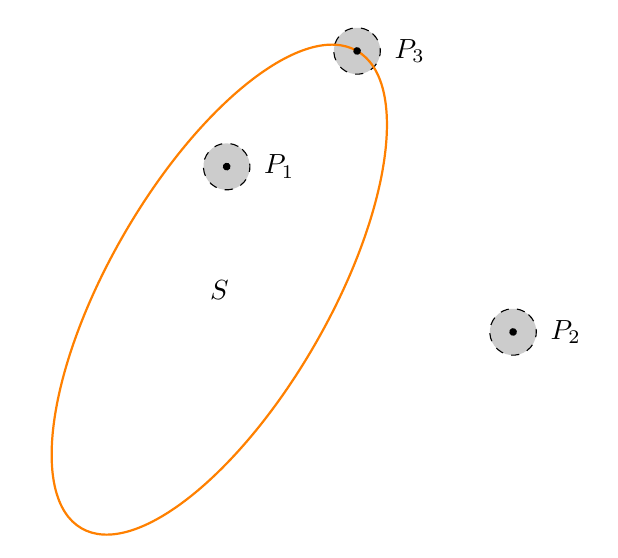
\begin{tikzpicture}[scale=.7]
\filldraw[rotate=60,draw=black,dashed,fill=gray!40]
	(2,1)circle(12pt)
	(2,-5)circle(12pt)
	(5,0)circle(12pt);
\draw[orange,rotate=60,thick](0,0)ellipse[x radius=5,y radius=2];
\draw (0,0)node{\(S\)};
\fill[rotate=60]
	(2,1)circle(2pt)node[right=10pt]{\(P_1\)}
	(2,-5)circle(2pt)node[right=10pt]{\(P_2\)}
	(5,0)circle(2pt)node[right=10pt]{\(P_3\)};
\end{tikzpicture}
\caption{平面上的点与点集的关系}
\label{figure:集合论.平面上的点与点集的关系}
\end{figure}
\end{definition}

\begin{property}
设点集\(S\subseteq\mathbb{R}^2\).
任意一点\(P\in\mathbb{R}^2\)要么是\(S\)的内点,要么是\(S\)的外点,要么是\(S\)的边界点.

换言之,任意点集\(S\)的内点、外点和边界点的集合均无交集,即:
\begin{enumerate}
\item \(I(S) \cap E(S) = \emptyset\).
\item \(\partial{S} \cap I(S) = \emptyset\).
\item \(\partial{S} \cap E(S) = \emptyset\).
\end{enumerate}
\end{property}

\begin{definition}
设点\(P\)和点集\(S\)满足\(P \in S\).
定义:若\(\exists \mathring{U}(P)\)使得\[
\mathring{U}(P) \cap S = \emptyset,
\]则称\(P\)为\(S\)的\textbf{孤立点}(acnode),记作\(P \in A(S)\).
\end{definition}

\begin{property}
\(S\)的内点必属于\(S\),即\[
P \in I(S) \implies P \in S
\]或\[
I(S) \subseteq S.
\]
\begin{proof}
\[
\left. \begin{array}{r}
P \in I(S) \iff \exists U(P) :\: U(P) \subseteq S \\
P \in U(P)
\end{array} \right\}
\implies P \in S.
\qedhere
\]
\end{proof}
\end{property}

\begin{property}
\(S\)的外点必不属于\(S\),即\(P \in E(S) \implies P \notin S\).
\begin{proof}
\begin{align*}
\left. \begin{array}{r}
P \in E(S) \iff \exists U(P) :\: U(P) \cap S = \emptyset \\
P \in U(P) \iff \{P\} \subseteq U(P) \implies \{P\} \cap S \subseteq U(P) \cap S
\end{array} \right\}
\implies& \{P\} \cap S \subseteq \emptyset \\
\implies \{P\} \cap S = \emptyset
\implies P \notin S.&
\qedhere
\end{align*}
\end{proof}
\end{property}

\begin{example}
点集的边界点可能属于该点集,也可能不属于它.例如,实轴上的左闭右开区间\([a,b)\)有两个边界点\(a\)和\(b\),但\(a \in [a,b)\)而\(b \notin [a,b)\).
\end{example}

\begin{definition}
设点\(P\in\mathbb{R}^2\),点集\(S\subseteq\mathbb{R}^2\).
定义:如果点\(P\)的任意邻域内总有\(S\)中的无穷多个点,则称\(P\)是\(S\)的\textbf{聚点}(Cluster),记作\(P \in C(S)\),即\[
P \in C(S)
\iff
\forall\delta>0,\exists Q \in S : Q \in \mathring{U}(P,\delta).
\]称点集\(S\)的聚点的集合\(C(S)\)为\(S\)的\textbf{导集}(derived set).
\end{definition}
任取点集\(S\)的一个聚点\(P_C\).由聚点的定义可知,\(P_C\)可以属于\(S\),也可以不属于\(S\).

\begin{theorem}
点\(P\)是点集\(S\)的聚点的充要条件是:在\(P\)的任意邻域内总有异于点\(P\)而属于\(S\)的一个点,即\[
\forall \delta>0 \bigl[
	\mathring{U}(P,\delta) \cap S \neq \emptyset
\bigr].
\]
\end{theorem}

\begin{property}
点集的内点均是其聚点,即\(I(S) \subseteq C(S)\).
\begin{proof}
由内点的定义有\(P \in I(S) \iff \exists \delta_1>0 :\: U(P,\delta_1) \subseteq S\).

当\(0 < \delta_2 \leqslant \delta_1\)时,有\[
\mathring{U}(P,\delta_2)
\subseteq U(P,\delta_1)
\subseteq S,
\]所以\[
\mathring{U}(P,\delta_2) \cap S
= \mathring{U}(P,\delta_2)
\neq \emptyset.
\]

当\(\delta_2 > \delta_1\)时,有\[
\emptyset \neq \mathring{U}(P,\delta_1) \subsetneqq U(P,\delta_1) \subseteq S,
\]\[
\mathring{U}(P,\delta_2) \cap S
\supseteq \mathring{U}(P,\delta_1) \cap S \neq \emptyset.
\]

综上所述,对于\(\forall \delta_2 > 0\)都有\(\mathring{U}(P,\delta_2) \cap S \neq \emptyset\)成立,即\(P \in C(S)\).
\end{proof}
\end{property}

\begin{property}
点集的外点不是其聚点,即\(P \in E(S) \implies P \notin C(S)\).
\begin{proof}
因为\(P \in E(S)\),所以\(\exists \delta > 0: U(P,\delta) \cap S = \emptyset\).又因为\(\mathring{U}(P,\delta) \subsetneqq U(P,\delta)\),所以\[
U(P,\delta) \cap S \supsetneqq \mathring{U}(P,\delta) \cap S = \emptyset,
\]从而有\(P \notin C(S)\).
\end{proof}
\end{property}

\begin{property}
点集的孤立点不是聚点,即\(P \in A(S) \implies P \notin C(S)\).
\begin{proof}
\(P \in A(S) \implies \exists \delta > 0 : \mathring{U}(P,\delta) \cap S = \emptyset \iff P \notin C(S)\).
\end{proof}
\end{property}

\begin{property}
点集的孤立点必不是其内点,点集的内点也必不是其孤立点,即\[
P \in A(S) \implies P \notin I(S),
\]\[
P \in I(S) \implies P \notin A(S).
\]
\end{property}

\begin{property}
点集的孤立点必不是其外点,点集的外点也必不是其孤立点,即\[
P \in A(S) \implies P \notin E(S),
\]\[
P \in E(S) \implies P \notin A(S).
\]
\end{property}

\begin{property}
点集的孤立点必是其边界点,即\(A(S) \subseteq \partial{S}\).
\end{property}

\begin{property}
点集的边界点可能是聚点,也可能不是聚点.
\end{property}

\begin{definition}
设点集\(S \subseteq \mathbb{R}^2\).

若\(S\)的点皆为它的内点,则称\(S\)为\textbf{开集}.若\(S\)的所有边界点都属于\(S\)(即\(\partial S \subseteq S\)),或所有聚点皆属于\(S\)(即\(C(S) \subseteq S\)),则称\(S\)为\textbf{闭集}.

若\(\exists r > 0\),使得\[
S \subseteq U(O,r),
\]其中\(O\)是坐标原点\(\opair{0,0}\),则称“\(S\)是\textbf{有界的}”或“\(S\)是\textbf{有界集}”;否则称“\(S\)是\textbf{无界的}”或“\(S\)是\textbf{无界集}”.

若\(S\)中任意两点均可用一条全含于\(S\)内的折线相连接,则称“\(S\)是\textbf{连通的}”或“\(S\)是\textbf{连通集}”.

若\(S\)既是连通集又是开集,则称\(S\)为\textbf{开区域}.开区域\(S\)及其边界\(\partial S\)的并集\(S + \partial S\)称为\textbf{闭区域}(简称\textbf{闭域},常记作\(\overline{S}\)).开区域与闭区域统称\textbf{区域}.

如果平面区域\(S\)内任一闭曲线所围的部分都属于\(S\),则称\(S\)为平面\textbf{单连通区域};否则称为平面\textbf{复连通区域}.
\end{definition}
